\subsection{Paketinio normalizavimo įtaka}
\label{subsec:rez_batch_norm}

Lyginamos dvi konfigūracijos – tinklas su paketinio normalizavimo (\textit{batch normalization}, BN) sluoksniais ir be jų. Rezultatai pateikti~\ref{tab:rez_batch_norm} lentelėje, validavimo metrikos – \ref{fig:rez_batch_norm_image} ir~\ref{fig:rez_batch_norm_keystroke} pav.

\begin{table}[H]
    \centering
    \caption{Paketinio normalizavimo tyrimo rezultatai. Geriausi variantai paryškinti.}
    \begin{tabular}{|l|l|c|c|c|}
        \hline
        Užduotis & Variantas & \texttt{val\_acc} & \texttt{val\_loss} & \texttt{test\_acc} \\
        \hline
        \multirow{2}{*}{Vaizdai}
            & Be BN     & $0{,}8360$ & $0{,}6696$ & $0{,}8432$ \\ \cline{2-5}
            & \textbf{Su BN} & $\mathbf{0{,}8942}$ & $\mathbf{0{,}3272}$ & $\mathbf{0{,}8602}$ \\
        \hline
        \multirow{2}{*}{Laiko eilutės}
            & Be BN     & $0{,}6750$ & $1{,}2623$ & $0{,}7167$ \\ \cline{2-5}
            & \textbf{Su BN} & $\mathbf{0{,}9167}$ & $\mathbf{0{,}2516}$ & $\mathbf{0{,}9033}$ \\
        \hline
    \end{tabular}
    \label{tab:rez_batch_norm}
\end{table}


\begin{figure}[H]
    \centering
    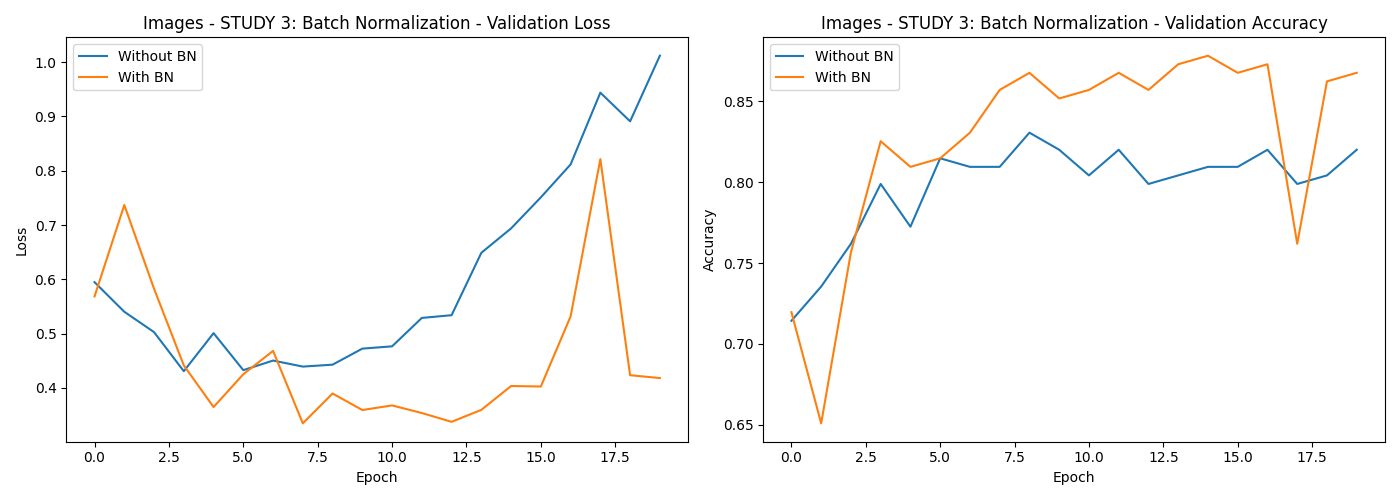
\includegraphics[width=0.9\linewidth]{3Lab/results/batch_norm/img_comparison.png}
    \caption{Paketinio normalizavimo tyrimas – vaizdų užduotis}
    \label{fig:rez_batch_norm_image}
\end{figure}

\begin{figure}[H]
    \centering
    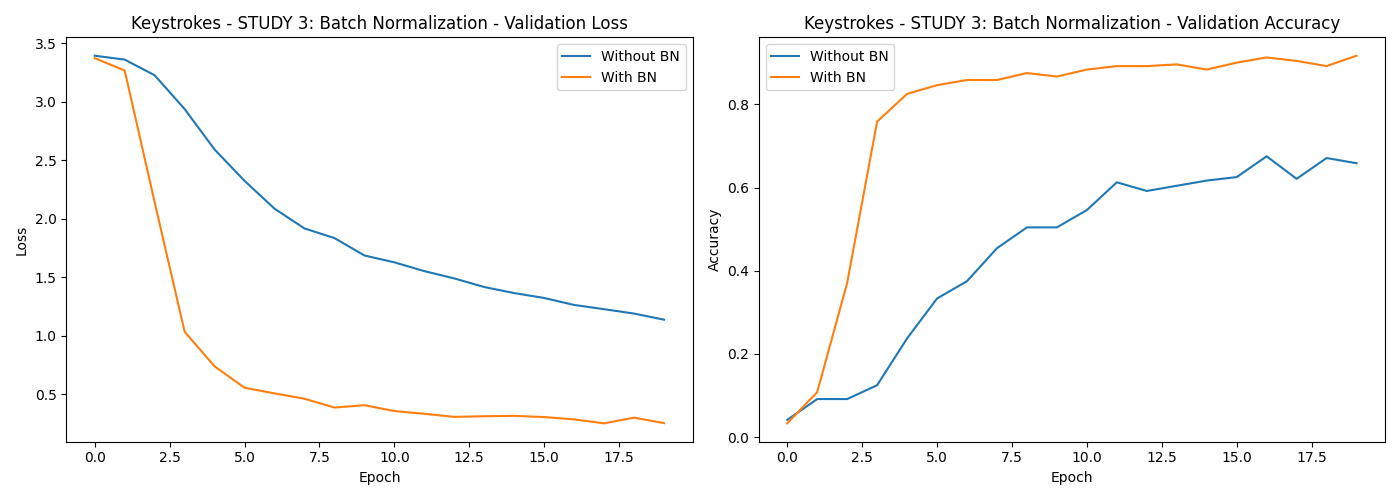
\includegraphics[width=0.9\linewidth]{3Lab/results/batch_norm/ks_comparison.png}
    \caption{Paketinio normalizavimo tyrimas – laiko eilučių užduotis}
    \label{fig:rez_batch_norm_keystroke}
\end{figure}

Pastebimi rezultatai:
\begin{itemize}
    \item BN sluoksniai \textbf{ryškiai pagerino abu modelius}: vaizdų \texttt{val\_acc} pakilo nuo $0{,}8360$ iki $0{,}8942$, laiko eilučių – nuo $0{,}6750$ iki $0{,}9167$.
    \item Validavimo paklaida sumažėjo apie $2 \times$, o validavimo tikslumas svyruoja gerokai mažiau – BN stabilizuoja mokymo procesą.
    \item Iš visų penkių tyrimų \textbf{BN konfigūracija} pasirodė geriausiai abiem užduotims, todėl ji parinkta galutiniam modelio įvertinimui (\ref{sec:geriausias_modelis} sk.).
\end{itemize}
